\section{Training Strategy and Data}
\label{sec:mllm_train}
A full-fledged MLLM undergoes three stages of training, \ie pre-training, instruction-tuning, and alignment tuning. Each phase of training requires different types of data and fulfills different objectives. In this section, we discuss training objectives, as well as data collection and characteristics for each training stage.

\subsection{Pre-training}
\label{sec:train_pre_train}

\subsubsection{Training Detail}
As the first training stage, pre-training mainly aims to align different modalities and learn multimodal world knowledge.
Pre-training stage generally entails large-scale text-paired data, \eg caption data. Typically, the caption pairs describe images/audio/videos in natural language sentences.

Here, we consider a common scenario where MLLMs are trained to align vision with text. As illustrated in~\cref{pretrain_prompt}, given an image, the model is trained to predict autoregressively the caption of the image, following a standard cross-entropy loss.
A common approach for pre-training is to keep pre-trained modules (\eg visual encoders and LLMs) frozen and train a learnable interface~\cite{detgpt, llava, llava-med}. The idea is to align different modalities without losing pre-trained knowledge. Some methods~\cite{mplug-owl,visionllm,bai2023qwen} also unfreeze more modules (\eg visual encoder) to enable more trainable parameters for alignment. 
It should be noted that the training scheme is closely related to the data quality. 
For short and noisy caption data, a lower resolution (\eg 224) can be adopted to speed up the training process, while for longer and cleaner data, it is better to utilize higher resolutions (\eg 448 or higher) to mitigate hallucinations. 
Besides, ShareGPT4V~\cite{chen2023sharegpt4v} finds that with high-quality caption data in the pretraining stage, unlocking the vision encode promotes better alignment. 

\begin{table}[!t]
\begin{tcolorbox}

Input: \textcolor[rgb]{0,0,0.8}{<image>}\ \par

Response: \textcolor[rgb]{0.8,0,0}{\{caption\}}

\end{tcolorbox}
\caption{A simplified template to structure the caption data. \textcolor[rgb]{0,0,0.8}{\{<image>\}} is the placeholder for the visual tokens, and \textcolor[rgb]{0.8,0,0}{\{caption\}} is the caption for the image. Note that only the part marked in \textcolor[rgb]{0.8,0,0}{red} is used for loss calculation.}
\label{pretrain_prompt}
\end{table}


\subsubsection{Data}
Pretraining data mainly serve two purposes, \ie (1) aligning different modalities and (2) providing world knowledge. 
The pretraining corpora can be divided into coarse-grained and fine-grained data according to granularities, which we will introduce sequentially. We summarize commonly used pretraining datasets in~\cref{tab:data-pretrain}.

Coarse-grained caption data share some typical traits in common: (1) The data volume is large since samples are generally sourced from the internet. (2) Because of the web-scrawled nature, the captions are usually short and noisy since they originate from the alt-text of the web images. 
These data can be cleaned and filtered via automatic tools, for example, using CLIP~\cite{clip} model to filter out image-text pairs whose similarities are lower than a pre-defined threshold.
In what follows, we introduce some representative coarse-grained datasets.


\noindent \textbf{CC.} 
CC-3M~\cite{CC} is a web-scale caption dataset of 3.3M image-caption pairs, where the raw descriptions are derived from alt-text associated with images. 
The authors design a complicated pipeline to clean data:
(1) For images, those with inappropriate content or aspect ratio are filtered. (2) For text, NLP tools are used to obtain text annotations, with samples filtered according to the designed heuristics. (3) For image-text pairs, images are assigned labels via classifiers. If text annotations do not overlap with image labels, the corresponding samples are dropped.

CC-12M~\cite{CC-12m} is a following work of CC-3M and contains 12.4M image-caption pairs. Compared with the previous work, CC-12M relaxes and simplifies the data-collection pipeline, thus collecting more data.

\noindent \textbf{SBU Captions~\cite{SBU-Captions}.} 
It is a captioned photo dataset containing 1M image-text pairs, with images and descriptions sourced from Flickr. 
Specifically, an initial set of images is acquired by querying the Flickr website with a large number of query terms. The descriptions attached to the images thus serve as captions. Then, to ensure that descriptions are relevant to the images, the retained images fulfill these requirements: (1) Descriptions of the images are of satisfactory length, decided by observation. (2) Descriptions of the images contain at least 2 words in the predefined term lists and a propositional word (\eg ``on'', ``under'') that generally suggests spatial relationships.

\noindent \textbf{LAION.}
This series are large web-scale datasets, with images scrawled from the internet and associated alt-text as captions. To filter the image-text pairs, the following steps are performed: (1) Text with short lengths or images with too small or too big sizes are dropped. (2) Image deduplication based on URL. (3) Extract CLIP~\cite{clip} embeddings for images and text, and use the embeddings to drop possibly illegal content and image-text pairs with low cosine similarity between embeddings.
Here we offer a brief summary of some typical variants:
\begin{itemize}[leftmargin=*]
    \item LAION-5B~\cite{laion-5b}: It is a research-purpose dataset of 5.85B image-text pairs. The dataset is multilingual with a 2B English subset.
    \item LAION-COCO~\cite{laion-coco}: It contains 600M images extracted from the English subset of LAION-5B. The captions are synthetic, using BLIP~\cite{li2022blip} to generate various image captions and using CLIP~\cite{clip} to pick the best fit for the image.
\end{itemize}


\begin{table}[!t]
\centering
\caption{Common datasets used for pre-training.}
\label{tab:data-pretrain}
\begin{tabular}{lcc}
\toprule
\textbf{Dataset}               & \textbf{Samples}   & \textbf{Date}             \\
\midrule
\multicolumn{3}{l}{\textbf{Coarse-grained Image-Text}}                             \\
\midrule
CC-3M~\cite{CC}                          & 3.3M                  & 2018                      \\
CC-12M~\cite{CC-12m}                         & 12.4M                 & 2020                      \\
SBU Captions~\cite{SBU-Captions}                   & 1M                    & 2011                      \\
LAION-5B~\cite{laion-5b}                       & 5.9B                  & Mar-2022                  \\
LAION-2B~\cite{laion-5b}                       & 2.3B                  & Mar-2022                  \\
LAION-COCO~\cite{laion-coco}                     & 600M                  & Sep-2022                  \\
COYO-700M~\cite{kakaobrain2022coyo-700m}                      & 747M                  & Aug-2022                  \\
\midrule
\multicolumn{3}{l}{\textbf{Fine-grained Image-Text}}                               \\
\midrule
ShareGPT4V-PT~\cite{chen2023sharegpt4v}    & 1.2M                & Nov-2023      \\
LVIS-Instruct4V~\cite{wang2023see}                & 111K                  & Nov-2023                  \\
ALLaVA~\cite{chen2024allava}                         & 709K                  & Feb-2024                  \\
\midrule
\multicolumn{3}{l}{\textbf{Video-Text}}                                            \\
\midrule
MSR-VTT~\cite{msr-vtt}                        & 200K                  & 2016                      \\
\midrule
\multicolumn{3}{l}{\textbf{Audio-Text}}                                            \\
\midrule
WavCaps~\cite{wavcaps}                        & 24K                   & Mar-2023            \\
\bottomrule
\end{tabular}
\end{table}


\noindent \textbf{COYO-700M~\cite{kakaobrain2022coyo-700m}.}
It contains 747M image-text pairs, which are extracted from CommonCrawl.
For data filtering, the authors design the following strategies:
(1) For images, those with inappropriate size, content, format, or aspect ratio are filtered. Moreover, the images are filtered based on the pHash value to remove images overlapped with public datasets such as ImageNet and MS-COCO. (2) For text, only English text with satisfactory length, noun forms, and appropriate words are saved. Whitespace before and after the sentence will be removed, and consecutive whitespace characters will be replaced with a single whitespace. Moreover, text appearing more than 10 times (\eg ``image for'') will be dropped. (3) For image-text pairs, duplicated samples are removed based on (image pHash, text) tuple.

Recently, more works~\cite{chen2023sharegpt4v,wang2023see,chen2024allava} have explored generating high-quality fine-grained data through prompting strong MLLMs (\eg GPT-4V). Compared with coarse-grained data, these data generally contain longer and more accurate descriptions of the images, thus enabling finer-grained alignment between image and text modalities. However, since this approach generally requires calling commercial-use MLLMs, the cost is higher, and the data volume is relatively smaller.  Notably, ShareGPT4V~\cite{chen2023sharegpt4v} strikes a balance by first training a captioner with GPT-4V-generated 100K data, then scaling up the data volume to 1.2M using the pre-trained captioner. 


\subsection{Instruction-tuning}
\label{sec:train_inst_tune}

\begin{figure}[t]
    \centering
    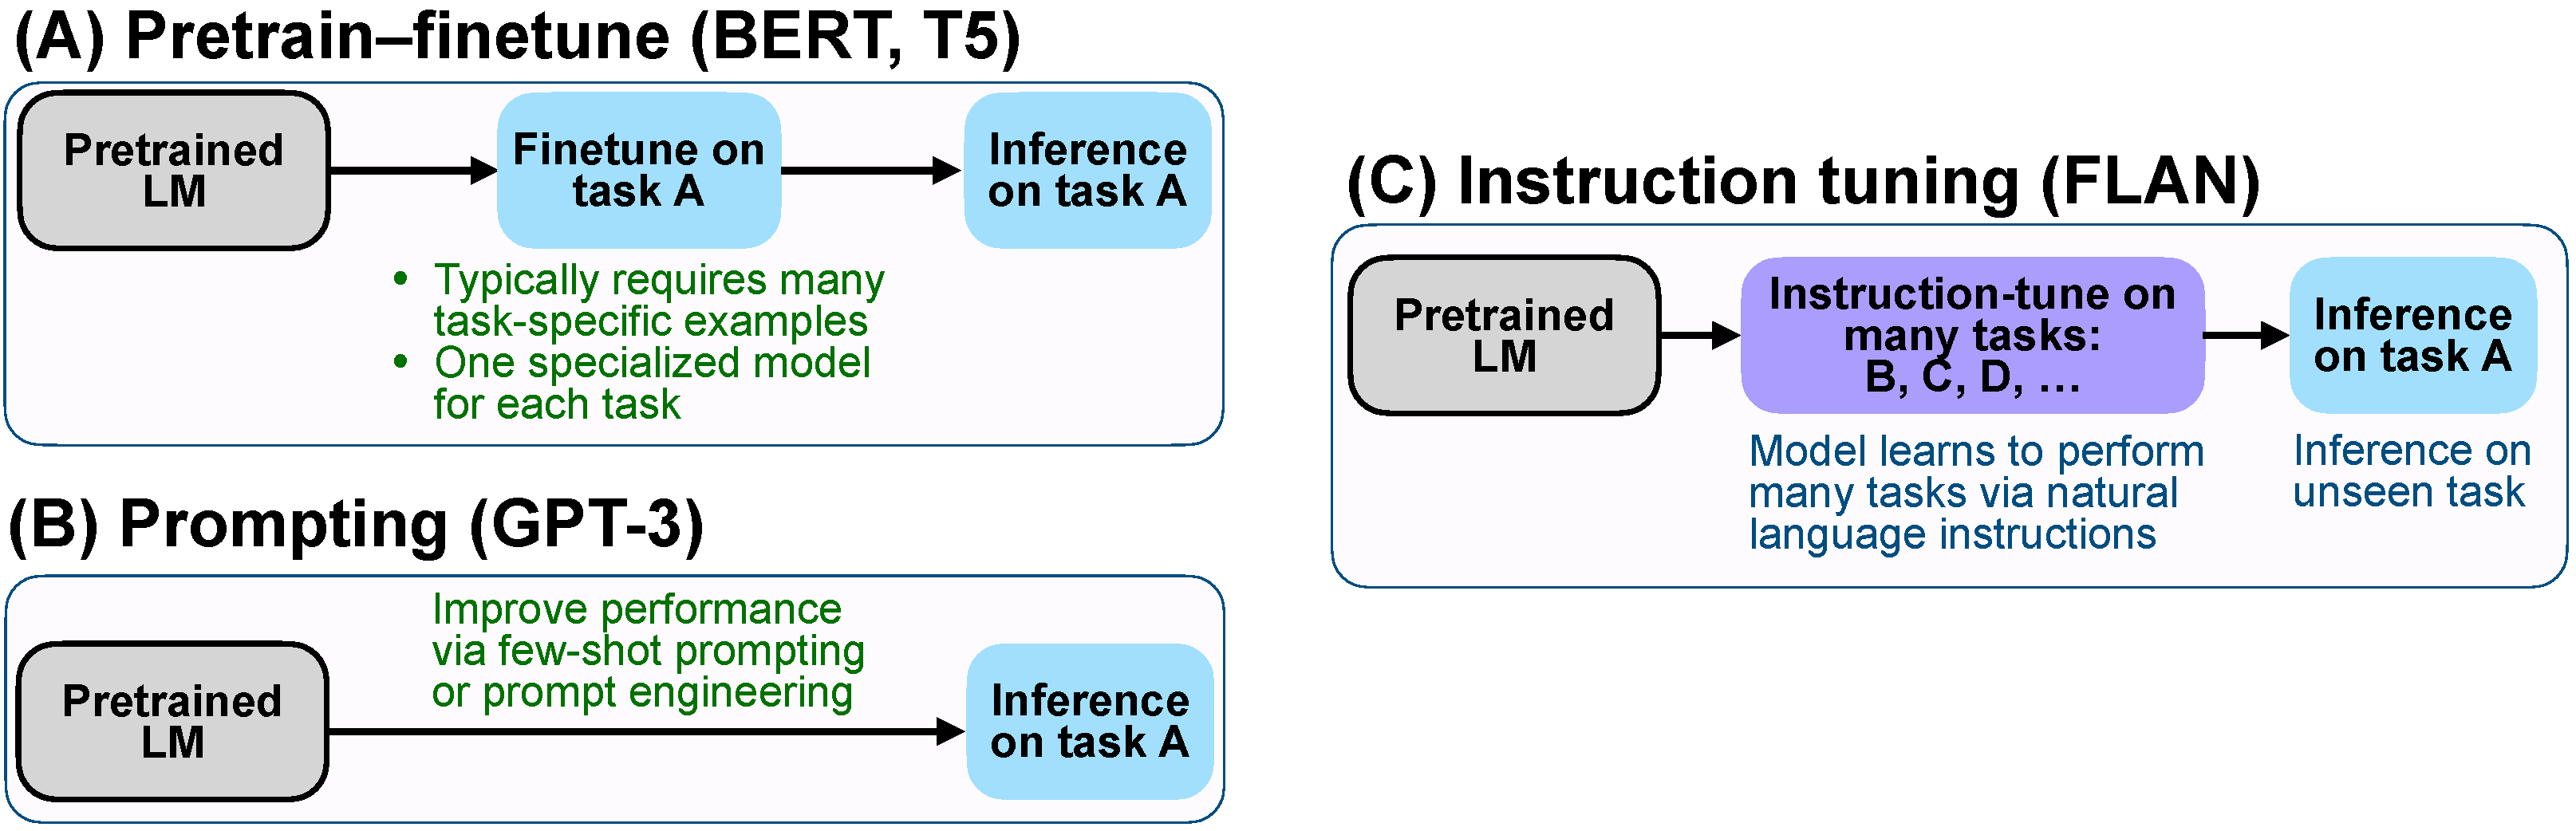
\includegraphics[width=0.985\linewidth]{figs/figure-compare-learn.pdf}
    \caption{Comparison of three typical learning paradigms. The image is from~\cite{wei2021finetuned}.}
    \label{fig:compare_learn}
\end{figure}

\subsubsection{Introduction}
Instruction refers to the description of tasks.
Intuitively, instruction tuning aims to teach models to better understand the instructions from users and fulfill the demanded tasks. 
Tuning in this way, LLMs can generalize to unseen tasks by following new instructions, thus boosting zero-shot performance. 
This simple yet effective idea has sparked the success of subsequent NLP works, such as ChatGPT~\cite{chatgpt}, InstructGPT~\cite{ouyang2022training}, FLAN~\cite{chung2022scaling, wei2021finetuned}, and OPT-IML~\cite{iyer2022opt}. 

The comparisons between instruction tuning and related typical learning paradigms are illustrated in \cref{fig:compare_learn}. 
The supervised fine-tuning approach usually requires a large amount of task-specific data to train a task-specific model.
The prompting approach reduces the reliance on large-scale data and can fulfill a specialized task via prompt engineering.
In such a case, though the few-shot performance has been improved, the zero-shot performance is still quite average~\cite{brown2020language}.
Differently, instruction tuning learns how to generalize to unseen tasks rather than fitting specific tasks like the two counterparts.
Moreover, instruction tuning is highly related to multi-task prompting~\cite{sanh2021multitask}.

In this section, we delineate the format of instruction samples, the training objectives, typical ways to gather instruction data, and corresponding commonly used datasets.


\subsubsection{Training Detail}
\label{sec:train_inst_tune_detail}


\begin{table}[!b]
\begin{tcolorbox}
Below is an instruction that describes a task. Write a response that appropriately completes the request \par\medskip

Instruction: \textcolor[rgb]{0,0,0.8}{<instruction>}

Input: \textcolor[rgb]{0,0,0.8}{\{<image>, <text>\}}\ 

Response: \textcolor[rgb]{0.8,0,0}{<output>}

\end{tcolorbox}
\caption{A simplified template to structure the multimodal instruction data. \textcolor[rgb]{0,0,0.8}{<instruction>} is a textual description of the task. \textcolor[rgb]{0,0,0.8}{\{<image>, <text>\}} and \textcolor[rgb]{0.8,0,0}{<output>} are input and output from the data sample. Note that \textcolor[rgb]{0,0,0.8}{<text>} in the input may be missed for some datasets, such as image caption datasets merely have \textcolor[rgb]{0,0,0.8}{<image>}. The example is adapted from~\cite{multimodal-gpt}.}
\label{vision_prompt}
\end{table}

A multimodal instruction sample often includes an optional instruction and an input-output pair. The instruction is typically a natural language sentence describing the task, such as, ``\textit{Describe the image in detail.}'' The input can be an image-text pair like the VQA task~\cite{antol2015vqa} or only an image like the image caption task~\cite{karpathy2015deep}. The output is the answer to the instruction conditioned on the input.
The instruction template is flexible and subject to manual designs~\cite{videochat, multimodal-gpt, llava}, as exemplified in \cref{vision_prompt}. Note that the instruction template can also be generalized to the case of multi-round conversations~\cite{multimodal-gpt, pmc-vqa, llava, pandagpt}.

Formally, a multimodal instruction sample can be denoted in a triplet form, \ie $(\mathcal{I}, \mathcal{M}, \mathcal{R})$, where $\mathcal{I}, \mathcal{M}, \mathcal{R}$ represent the instruction, the multimodal input, and the ground truth response, respectively. The MLLM predicts an answer given the instruction and the multimodal input:
\begin{equation}
    \mathcal{A} = f(\mathcal{I}, \mathcal{M}; \theta)
\end{equation}
Here, $\mathcal{A}$ denotes the predicted answer, and $\theta$ are the parameters of the model. 
The training objective is typically the original auto-regressive objective used to train LLMs~\cite{llava, pmc-vqa, pandagpt, lavin}, based on which the MLLM is encouraged to predict the next token of the response. The objective can be expressed as:
\begin{equation}
\mathcal{L}(\theta) = -\sum_{i=1}^{N} \log p(\mathcal{R}_i|\mathcal{I}, \mathcal{R}_{<i}; \theta)
\end{equation}
where $N$ is the length of the ground-truth response. 

\subsubsection{Data Collection}
\label{sec:train_inst_tune_collect}
Since instruction data are more flexible in formats and varied in task formulations, it is usually trickier and more costly to collect data samples. In this section, we summarize three typical ways to harvest instruction data at scale, \ie data adaptation, self-instruction, and data mixture.

\begin{table*}[!htbp]
\begin{tcolorbox}
\centering
\small
\begin{itemize}[leftmargin=2.5mm]
\setlength{\itemsep}{1pt}
\item <Image> \{Question\}
\item <Image> Question: \{Question\}
\item <Image> \{Question\} A short answer to the question is
\item <Image> Q: \{Question\} A:
\item <Image> Question: \{Question\} Short answer:
\item <Image> Given the image, answer the following question with no more than three words. \{Question\}
\item <Image> Based on the image, respond to this question with a short answer: \{Question\}. Answer:
\item <Image> Use the provided image to answer the question: \{Question\} Provide your answer as short as possible:
\item <Image> What is the answer to the following question? "\{Question\}"
\item <Image> The question "\{Question\}" can be answered using the image. A short answer is
\end{itemize}
\end{tcolorbox}
\caption{Instruction templates for VQA datasets, cited from~\cite{instructblip}. <Image> and \{Question\} are the image and the question in the original VQA datasets, respectively.}
\label{tab:vqa_instructions}
\end{table*}

\noindent \textbf{Data Adaptation.}
Task-specific datasets are rich sources of high-quality data. Hence, abundant works~\cite{instructblip, visionllm, x-llm, multiinstruct, llama-adapter, llama-adapter-v2, chatbridge, lavin} have utilized existing high-quality datasets to construct instruction-formatted datasets. Take the transformation of VQA datasets for an example, the original sample is an input-out pair where the input comprises an image and a natural language question, and the output is the textual answer to the question conditioned on the image. The input-output pairs of these datasets could naturally comprise the multimodal input and response of the instruction sample (see \S\ref{sec:train_inst_tune_detail}). The instructions, \ie the descriptions of the tasks, can either derive from manual design or from semi-automatic generation aided by GPT. Specifically, some works~\cite{instructblip, multiinstruct, minigpt-4, x-llm, llava-med, m3it} hand-craft a pool of candidate instructions and sample one of them during training. We offer an example of instruction templates for the VQA datasets as shown in~\cref{tab:vqa_instructions}. The other works manually design some seed instructions and use these to prompt GPT to generate more~\cite{visionllm, videochat, multimodal-gpt}. 

Note that since the answers of existing VQA and caption datasets are usually concise, directly using these datasets for instruction tuning may limit the output length of MLLMs. There are two common strategies to tackle this problem. 
The first one is to specify explicitly in instructions. 
For example, ChatBridge~\cite{chatbridge} explicitly declares \textit{short} and \textit{brief} for short-answer data, as well as \textit{a sentence} and \textit{single sentence} for conventional coarse-grained caption data.
The second one is to extend the length of existing answers~\cite{m3it}.
For example, M$^3$IT~\cite{m3it} proposes to rephrase the original answer by prompting ChatGPT with the original question, answer, and contextual information of the image (\eg caption and OCR).



\begin{table*}[!htb]
\centering
\caption{A summary of popular datasets generated by self-instruction. For input/output modalities, I: Image, T: Text, V: Video, A: Audio. For data composition, M-T and S-T denote multi-turn and single-turn, respectively.}
\label{tab:IT-data}
\begin{tabular}{lcccc}
\toprule
\textbf{Dataset} & \textbf{Sample} & \textbf{Modality}     & \textbf{Source} & \textbf{Composition}                     \\
\midrule
LLaVA-Instruct   & 158K              & I + T $\rightarrow$ T & MS-COCO         & 23K caption + 58K M-T QA + 77K reasoning \\
LVIS-Instruct & 220K & I + T $\rightarrow$ T & LVIS         & 110K caption + 110K M-T QA             \\
ALLaVA        & 1.4M & I + T $\rightarrow$ T & VFlan, LAION & 709K caption + 709K S-T QA             \\
\midrule
Video-ChatGPT & 100K & V + T $\rightarrow$ T & ActivityNet  & 7K description + 4K M-T QA             \\
VideoChat     & 11K  & V+T $\rightarrow$ T   & WebVid       & description + summarization + creation \\
\midrule
Clotho-Detail & 3.9K & A + T $\rightarrow$ T & Clotho       & caption                                \\
\bottomrule
\end{tabular}
\end{table*}



\noindent \textbf{Self-Instruction.}
Although existing multi-task datasets can contribute a rich source of data, they usually do not meet human needs well in real-world scenarios, such as multiple rounds of conversations.
To tackle this issue, some works collect samples through self-instruction~\cite{wang2022self}, which utilizes LLMs to generate textual instruction-following data using a few hand-annotated samples. Specifically, some instruction-following samples are hand-crafted as demonstrations, after which ChatGPT/GPT-4 is prompted to generate more instruction samples with the demonstrations as guidance. LLaVA~\cite{llava} extends the approach to the multimodal field by translating images into text of captions and bounding boxes, and prompting text-only GPT-4 to generate new data with the guidance of requirements and demonstrations. 
In this way, a multimodal instruction dataset is constructed, called LLaVA-Instruct-150k. Following this idea, subsequent works such as MiniGPT-4~\cite{minigpt-4}, ChatBridge~\cite{chatbridge}, GPT4Tools~\cite{gpt4tools}, and DetGPT~\cite{detgpt} develop different datasets catering for different needs.
Recently, with the release of the more powerful multimodal model GPT-4V, many works have adopted GPT-4V to generate data of higher quality, as exemplified by LVIS-Instruct4V~\cite{wang2023see} and ALLaVA~\cite{chen2024allava}. We summarize the popular datasets generated through self-instruction in~\cref{tab:IT-data}.


\noindent \textbf{Data Mixture.}
Apart from the multimodal instruction data, language-only user-assistant conversation data can also be used to improve conversational proficiencies and instruction-following abilities~\cite{llama-adapter-v2, mplug-owl, multimodal-gpt, lavin}. 
LaVIN~\cite{lavin} directly constructs a minibatch by randomly sampling from both language-only and multimodal data. 
MultiInstruct~\cite{multiinstruct} probes different strategies for training with a fusion of single modal and multimodal data, including mixed instruction tuning (combine both types of data and randomly shuffle) and sequential instruction tuning (text data followed by multimodal data).


\subsubsection{Data Quality}
Recent research has revealed that the data quality of instruction-tuning samples is no less important than quantity.
Lynx~\cite{zeng2023matters} finds that models pre-trained on large-scale but noisy image-text pairs do not perform as well as models pre-trained with smaller but cleaner datasets.
Similarly, Wei~\etal~\cite{wei2023instructiongpt} finds that less instruction-tuning data with higher quality can achieve better performance. For data filtering, the work proposes some metrics to evaluate data quality and, correspondingly, a method to automatically filter out inferior vision-language data.
Here we discuss two important aspects regarding data quality.  

\noindent \textbf{Prompt Diversity.}
The diversity of instructions has been found to be critical for model performance. Lynx~\cite{zeng2023matters} empirically verifies that diverse prompts help improve model performance and generalization ability. 

\noindent \textbf{Task Coverage.}
In terms of tasks involved in training data, Du~\etal~\cite{du2023makes} perform an empirical study and find that the visual reasoning task is superior to captioning and QA tasks for boosting model performance. Moreover, the study suggests that enhancing the complexity of instructions might be more beneficial than increasing task diversity and incorporating fine-grained spatial annotations.


\subsection{Alignment tuning}
\label{sec:train_align_tune}

\subsubsection{Introduction}
Alignment tuning is more often used in scenarios where models need to be aligned with specific human preferences, \eg response with fewer hallucinations (see \S \ref{sec:hallu}).
Currently, Reinforcement Learning with Human Feedback (RLHF) and Direct Preference Optimization (DPO) are two main techniques for alignment tuning. In this section, we introduce the main ideas of the two techniques in sequence and offer some examples of how they are utilized in addressing practical problems, and finally, give a compilation of the related datasets.

\subsubsection{Training Detail}

\noindent \textbf{RLHF~\cite{ziegler2019fine, stiennon2020learning}.}
This technique aims to utilize reinforcement learning algorithms to align LLMs with human preferences, with human annotations as supervision in the training loop. As exemplified in InstructGPT~\cite{ouyang2022training}, RLHF incorporates three key steps:

\begin{enumerate}[leftmargin=*]
    \item \textbf{Supervised fine-tuning.} This step aims to fine-tune a pre-trained model to present the preliminary desired output behavior. The fine-tuned model in the RLHF setting is called a \textit{policy model}. Note that this step might be skipped since the supervised policy model $\pi^{\text{SFT}}$ can be initialized from an instruction-tuned model (see \S \ref{sec:train_inst_tune}). 
    \item \textbf{Reward modeling.} A \textit{reward model} is trained using preference pairs in this step. Given a multimodal prompt (\eg image and text) $x$ and a response pair $(y_w, y_l)$, the reward model $r_\theta$ learns to give a higher reward to the preferred response $y_w$, and vice versa for $y_l$, according to the following objective:
    \begin{equation}
        \mathcal{L}(\theta)=-\mathbb{E}_{(x,y_w,y_l)\sim \mathcal{D}} \left[ \log (\sigma(r_\theta (x, y_w) - r_\theta(x, y_l) \right]
    \end{equation}
    where $\mathcal{D}=\{(x,y_w,y_l)\}$ is the comparison dataset labeled by human annotators. In practice, the reward model $r_\theta$ shares a similar structure with the policy model.
    \item \textbf{Reinforcement learning.} In this step, the Proximal Policy Optimization (PPO) algorithm is adopted to optimize the RL policy model $\pi^{\text{RL}}_\phi$. A per-token KL penalty is often added to the training objective to avoid deviating too far from the original policy~\cite{ouyang2022training}, resulting in the objective:
     \begin{equation}
     \begin{split}
        \mathcal{L}(\phi) &= -\mathbb{E}_{x\sim \mathcal{D}, y\sim \pi^{RL}_{\phi}(y|x)} \Big[ r_\theta(x,y)  \\
        &- \beta\cdot \mathbb{D}_{KL}\Big(\pi^{RL}_{\phi}(y|x) || \pi^{REF}(y|x)\Big) \Big]
    \end{split}
    \end{equation}
    where $\beta$ is the coefficient for the KL penalty term. Typically, both the RL policy $\pi^{\text{RL}}_\phi$ and the reference model $\pi^{\text{REF}}$ are initialized from the supervised model $\pi^{\text{SFT}}$. The obtained RL policy model is expected to align with human preferences through this tuning process.    
\end{enumerate}

Researchers have explored using the RLHF techniques for better multimodal alignment. For example, LLaVA-RLHF~\cite{sun2023aligning} collects human preference data and tunes a model with fewer hallucinations based on LLaVA~\cite{llava}.

\noindent \textbf{DPO~\cite{rafailov2023direct}.}
It learns from human preference labels utilizing a simple binary classification loss. Compared with the PPO-based RLHF algorithm, DPO is exempt from learning an explicit reward model, thus simplifying the whole pipeline to two steps, \ie human preference data collection and preference learning. The learning objective is as follows:
\begin{equation}
\begin{split}
    \mathcal{L}(\phi) &= -\mathbb{E}_{(x,y_w,y_l)\sim \mathcal{D}} \Big[ \log \sigma\Big( \beta \log \frac{\pi_\phi^{\text{RL}}(y_w|x)}{\pi^{\text{REF}}(y_w|x)} \\ 
    &- \beta \log \frac{\pi_\phi^{\text{RL}}(y_l|x)}{\pi^{\text{REF}}(y_l|x)} \Big)\Big]
\end{split}
\end{equation}
RLHF-V~\cite{yu2023rlhf} collects fine-grained (segment-level) preference data pairs by correcting hallucinations in the model response and uses the obtained data to perform dense DPO.
Silkie\cite{li2023silkie} instead collects preference data via prompting GPT-4V and distills the preference supervision into an instruction-tuned model through DPO.

\subsubsection{Data}
The gist of data collection for alignment-tuning is to collect feedback for model responses, \ie to decide which response is better. 
It is generally more expensive to collect such data, and the amount of data used for this phase is typically even less than that used in previous stages. 
In this part, we introduce some datasets and summarize them in~\cref{tab:align-tune-data}.

\noindent \textbf{LLaVA-RLHF~\cite{sun2023aligning}.}
It contains 10K preference pairs collected from human feedback in terms of honesty and helpfulness. The dataset mainly serves to reduce hallucinations in model responses.

\noindent \textbf{RLHF-V~\cite{yu2023rlhf}.}
It has 5.7K fine-grained human feedback data collected by segment-level hallucination corrections.

\noindent \textbf{VLFeedback~\cite{li2023silkie}.}
It utilizes AI to provide feedback on model responses. The dataset contains more than 380K comparison pairs scored by GPT-4V in terms of helpfulness, faithfulness, and ethical concerns. 


\begin{table}[!t]
\centering
\caption{A summary of datasets for alignment-tuning. For input/output modalities, I: Image, T: Text.}
\label{tab:align-tune-data}
\begin{tabular}{lccc}
\toprule
\textbf{Dataset} & \textbf{Sample} & \textbf{Modality}     & \textbf{Source} \\
\midrule
LLaVA-RLHF~\cite{sun2023aligning}       & 10K               & I + T $\rightarrow$ T & Human           \\
RLHF-V~\cite{yu2023rlhf}           & 5.7K              & I + T $\rightarrow$ T & Human           \\
VLFeedback~\cite{li2023silkie}       & 380K              & I + T $\rightarrow$ T & GPT-4V          \\
\bottomrule
\end{tabular}
\end{table}

